% 拍频
% 简谐振动|频率|拍频

\pentry{简谐振子\upref{SHO}}

\subsection{同一直线上两个不同频率的谐振动的合成}

设一质点在一直线上同时参与两个不同频率的谐振动,其振动表达式为
\begin{equation}
\begin{array}{l}x_{1}=A_{1} \cos \left(\omega_{1} t+\phi_{01}\right) \\ x_{2}=A_{2} \cos \left(\omega_{2} t+\phi_{02}\right)\end{array}
\end{equation}
根据叠加原理,合运动的位移为
\begin{equation}
x=x_{1}+x_{2}=A_{1} \cos \left(\omega_{1} t+\phi_{01}\right)+A_{2} \cos \left(\omega_{2} t+\phi_{02}\right)
\end{equation}

为方便计算,设$A_1=A_2=A,\phi_{01}=\phi_{02}=\phi_{0}$,则上式可化成
\begin{equation} \label{beatno_eq1}
x=2 A \cos \left(\frac{\omega_{2}-\omega_{1}}{2} t\right) \cos \left(\frac{\omega_{2}+\omega_{1}}{2} t+\phi_{0}\right)
\end{equation}
对于通常实际遇到的情况而言,两个频率比较接近,且$\left|\omega_{2}-\omega_{1}\right|\ll \omega_1$,\autoref{beatno_eq1}中第一项因子随时间作缓慢地变化,第二项因子是角频率近于$\omega$(即接近于$\omega_1,\omega_2$)的简谐函数,因此合成的振动可近似看成是角频率为$(\omega_{1}+\omega_{2})/2 \approx \omega_{1} \approx \omega_{2}$,振幅为$\left | 2 A \cos (\omega_{2}-\omega_{1})t/{2} \right |$的谐振动.这种两个频率较大且差值较小的谐振动合成时,合振幅出现时强时弱周期性缓慢变化的现象,叫做\textbf{拍(beat)}.

\begin{figure}[ht]
\centering
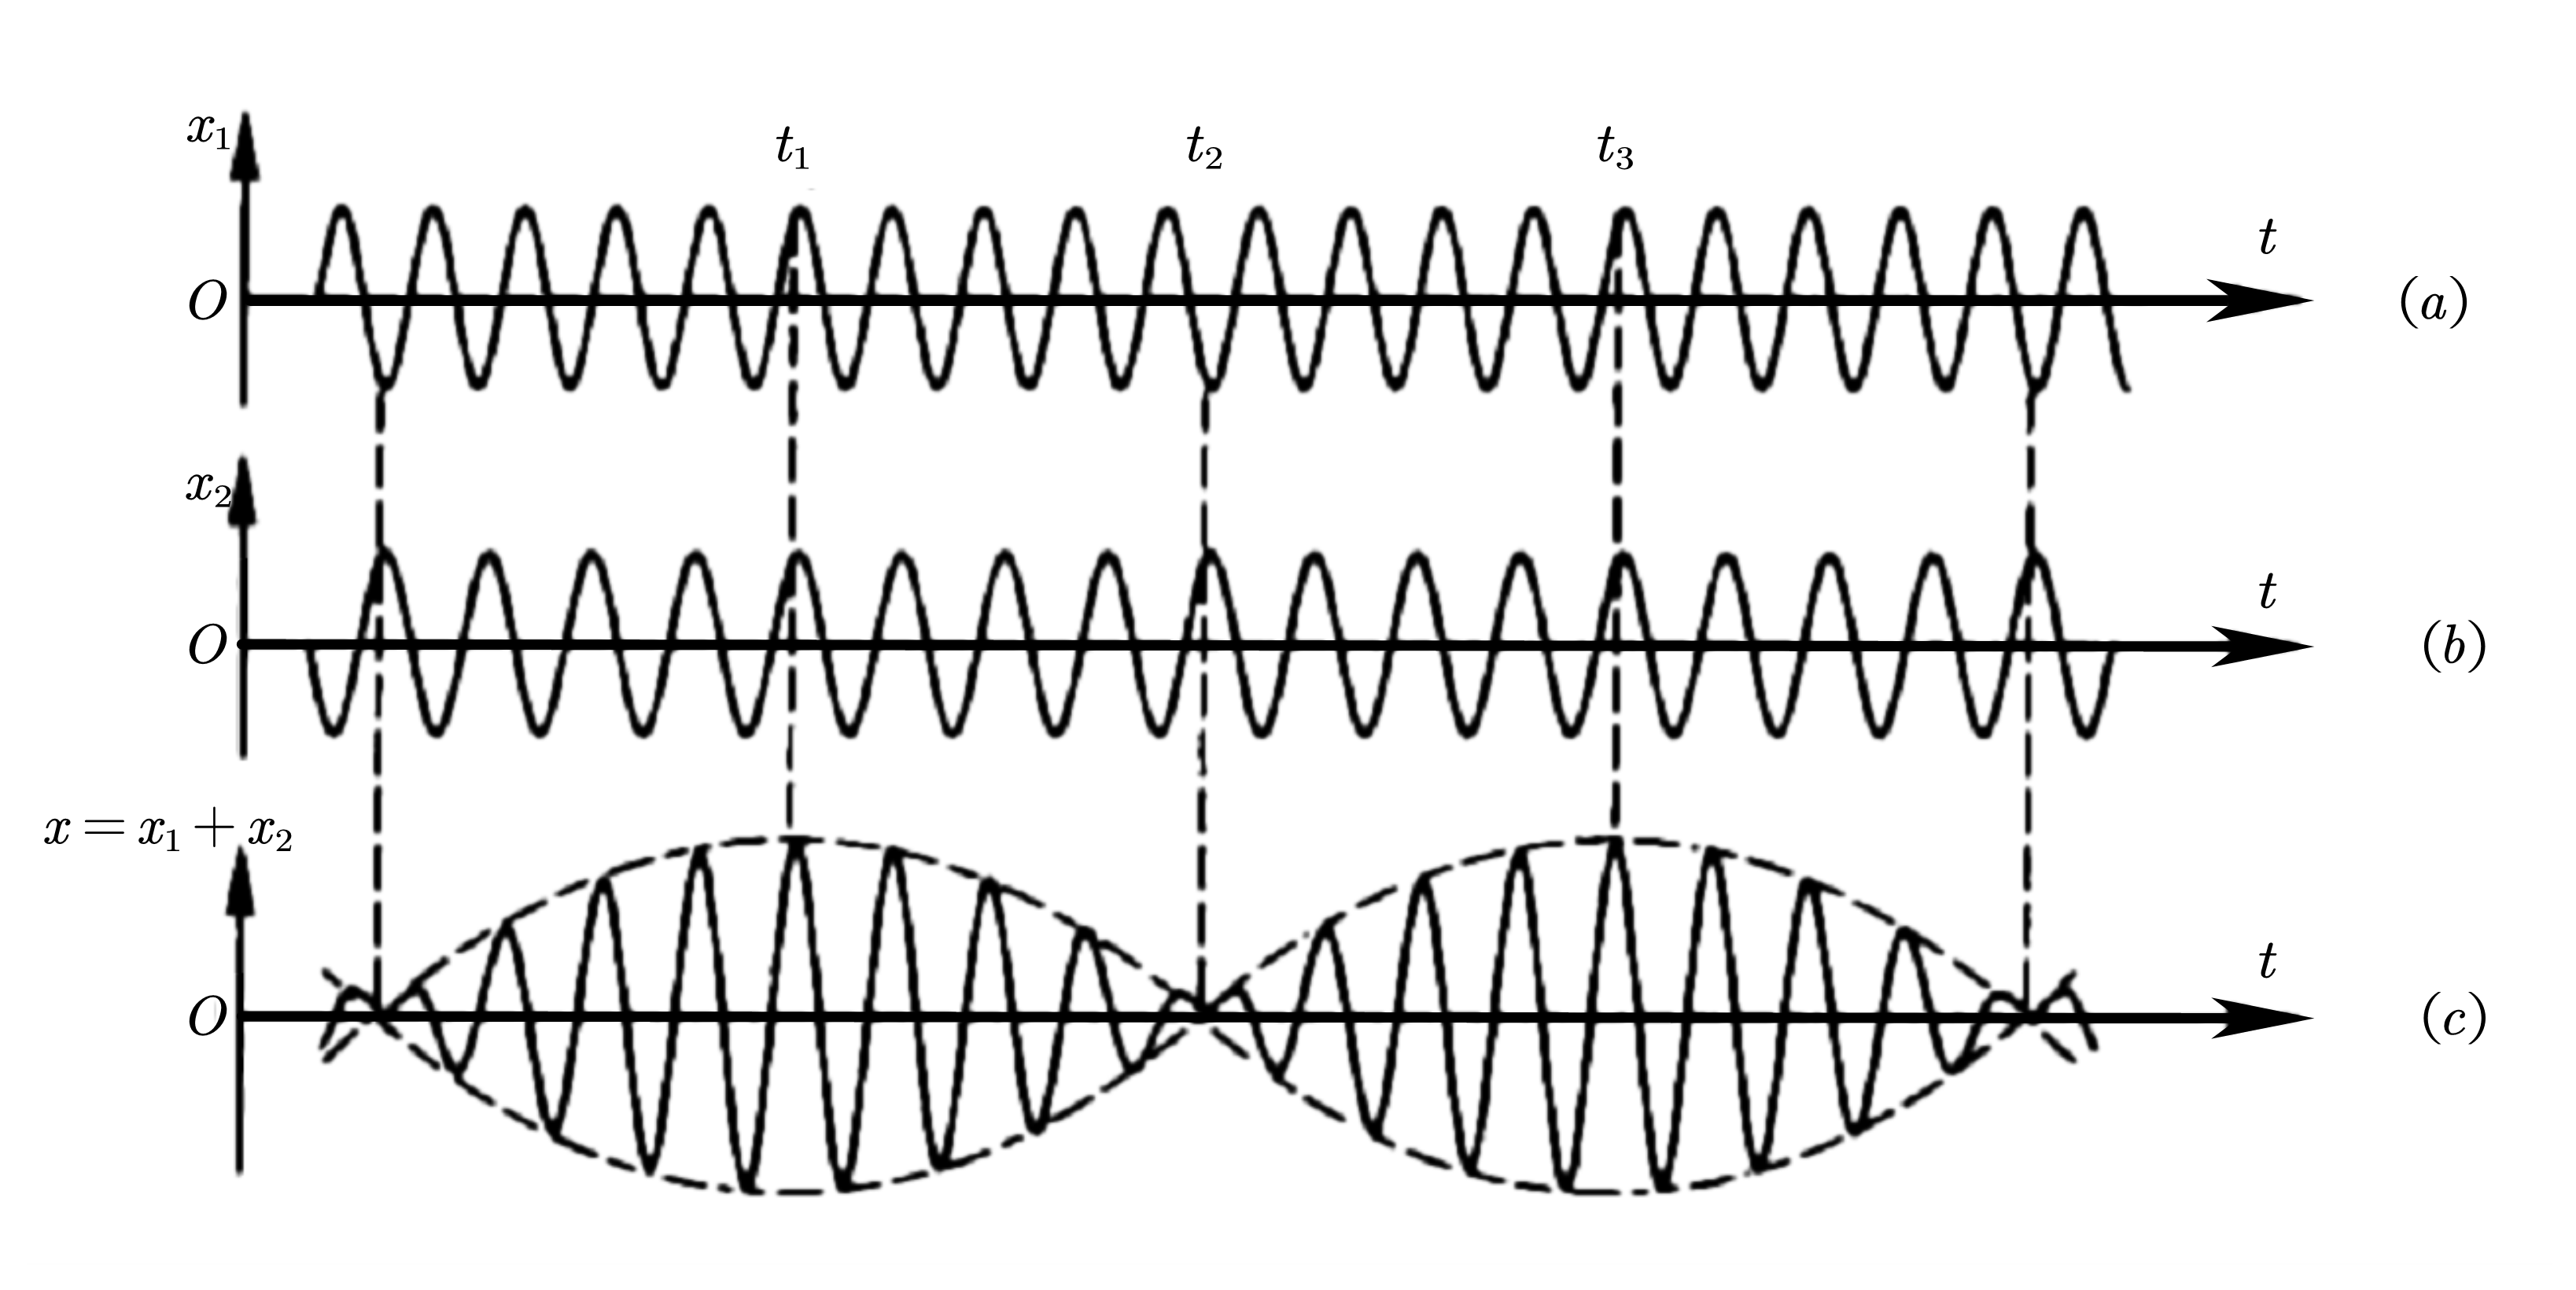
\includegraphics[width=13cm]{./figures/beatno_1.png}
\caption{拍} \label{beatno_fig1}
\end{figure}

拍出现的频率叫做\textbf{拍频}, 等于两分振动频率之差.

拍现象在技术上有重要应用.例如,管乐器中的双簧管就是利用两个簧片振动频率的微小差别产生颤动的拍音;调整乐器时,使它和标准音叉出现的拍音消失来校准乐器;拍现象常用于汽车速度监视器、地面卫星跟踪等.此外,在各种电子学测量仪器中,也常常用到拍现象.